% Chapter 2

\chapter{DSL Specification with CINCO}\label{ch:DSL}
This chapter explains the specification underlying the user documentation model. A \acrshort{dsl}, as the name suggests, is a language adapted to specific development domain. In our case, the specification is a textual DSL used to generate the graphical model element. The chapter starts by giving a overview of the framework in use and the boilerplate code coming with it. It then continues with the main aspects of the meta graph language and the meta style language as well as the cinco product definition. Finally, important key points of the Xtend generator classes are provided.
\section{CINCO SCCE Meta Tooling Framework}\label{sec:CTF}
The CINCO Framework is one of the many projects of the SCCE Group, which aims at allowing the application experts, rather than programming experts, to take charge of the development tasks~\cite{scce}. It is a generator-driven development environment for graphical domain-specific modeling tools. As for many software frameworks, the purpose to ease the development process by hiding the complexity of the underlying APIs and also by offering a selective integration of custom user-written code. Hence, it is reusable and application specific. The framework is based on the Eclipse Modeling Framework (EMF) and Graphiti Graphical Tooling Infrastructure~\cite{Cinco}. The widely spread Eclipse's Integrated Development Environment (IDE) provides the necessary support and a certain familiarity with the editor, which makes it easy to use for software development.
\begin{figure}[h]
    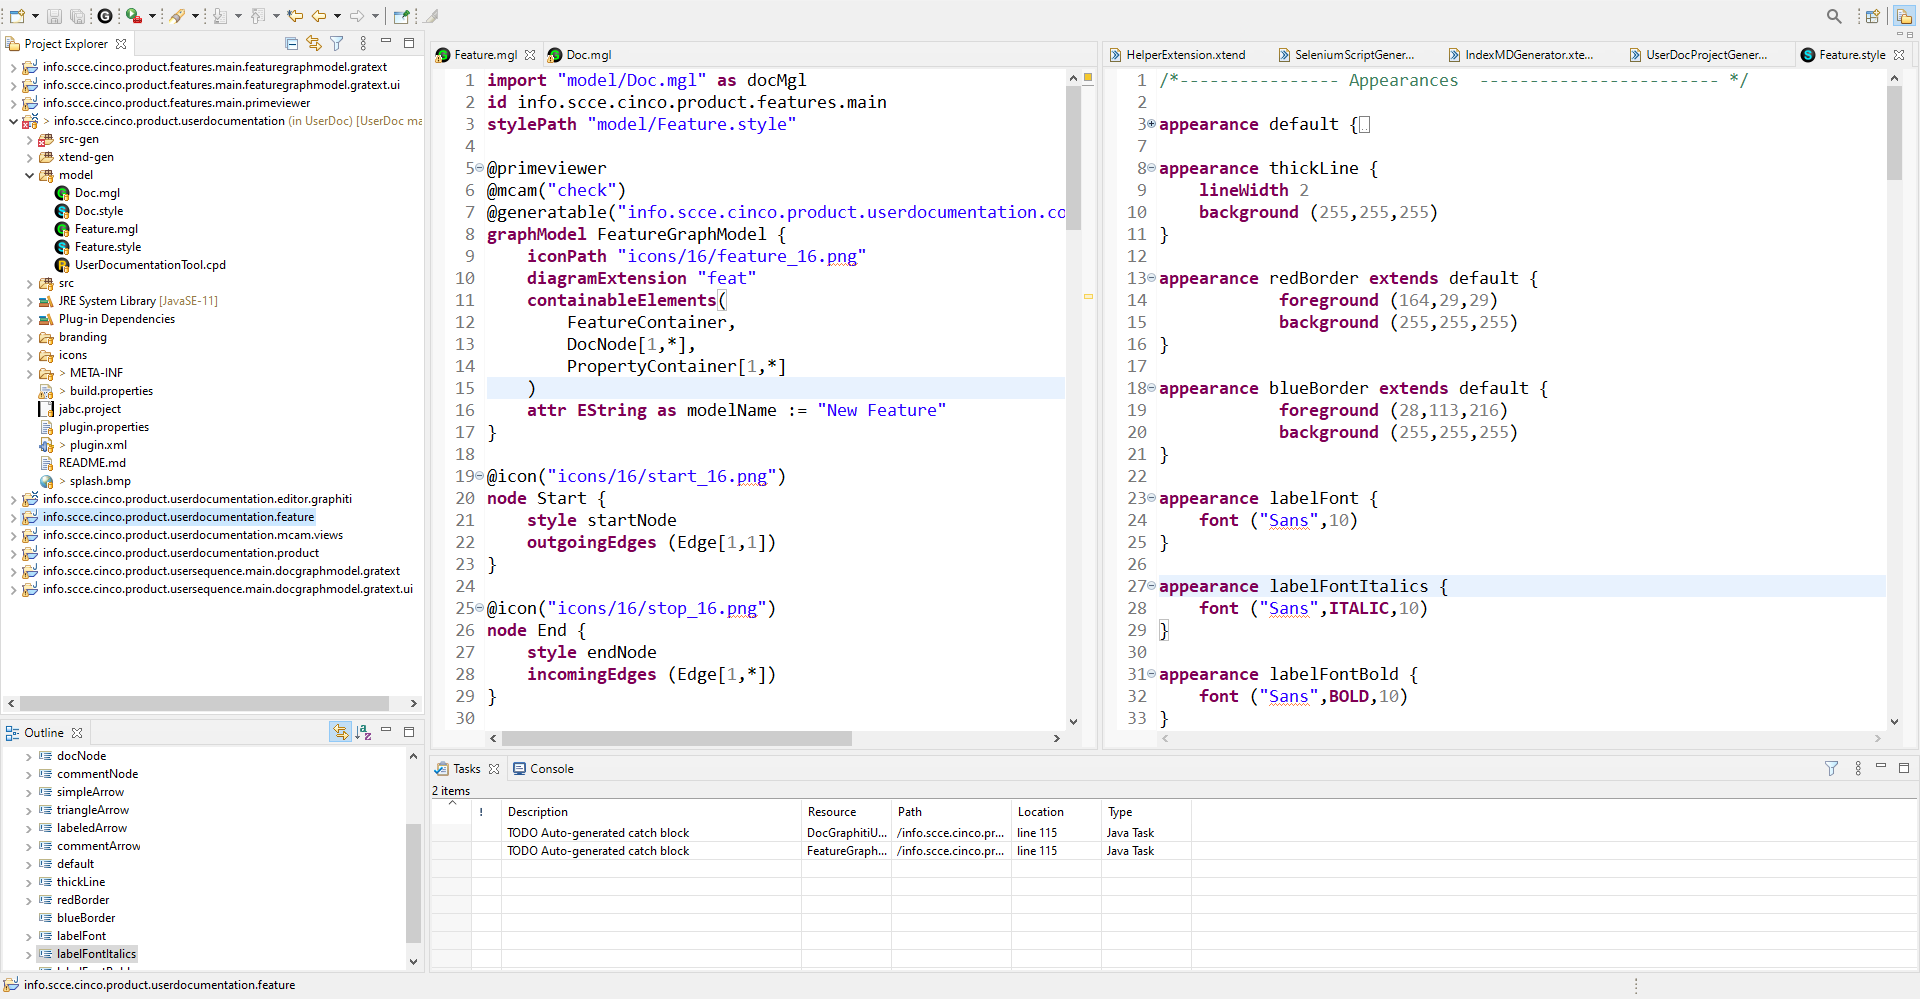
\includegraphics[width=\textwidth]{Cinco_EMF-Editor}
    \caption{The look of the CINCO IDE based on Eclipse}
\end{figure}

The term \textit{Meta} indicates that the tooling suite proposes a solution for the meta-specification of the corresponding domain-specific modeling tool. That means, the developer specifies the behavior and restrictions of the resulting graphical domain-specific modeling tool. Applying the concept of specialization at higher level brings much more control over the definition of the modeling tool and hence simplifies the development process. In this regard, the CINCO framework offers a push-button generation at meta-specification level for the creation of the graphical tool editor~\cite{scce}. The generated editor instance is also an Eclipse-based editor, that can as well generate and execute programs on its turn, based on the tailored graphical model.

Xtext is used to define the textual syntax of the meta-specification that defines the appearance and structure of the model elements. This will not be discuss further as this will extrapolate the context of the thesis.  \textit{'Implementing Domain-Specific Languages with Xtext and Xtend'} by Lorenzo Bettini is a good reference to read more about use of Xtext in DSL development. On the official \href{https://www.eclipse.org/Xtext/}{Eclipse website}, Xtext is defined as an open source framework for development of programming languages and domain-specific languages. Section \hyperref[sec:MGL]{2.2}, \hyperref[sec:MSL]{2.3} and \hyperref[sec:CPD]{2.4} will offer an in-depth explanation on how this \acrshort{dsl} syntax is used to determine the look of each model element.

With each generation an Ecore object specific to each tool is also created to provide a description for the model and support needed at runtime. Ecore stands for \textit{\acrfull{emf} core}, which is the meta model included in that framework. In addition, a corresponding editor based on Graphiti framework as well. It enables the creation, visualization and manipulation of the resulting model elements. Like most framework used in CINCO, Graphiti is also build around the \acrshort{emf} to allow the creation of diagram editors for targeted graphical domain models. More about Graphiti can be found \href{https://www.eclipse.org/graphiti/}{here}.

The full generation process of a graphical modeling tool (of a CINCO Product Application) comprises four essential (meta-) levels~\cite{Naujokat2018}. The first level, associated with the role Eclipse Developer, is where the Ecore.ecore and GraphitiDiagram.ecore meta model are developed. The second level is where CINCO Developers of the Chair 5 for Programming Systems used the aforementioned meta model to develope the MGL.ecore and Style.ecore (actually corresponding to the MSL described in Sec. \hyperref[sec:MSL]{2.3}), which in turns will become meta model of the third specification level, where the CINCO Product Developers operate. This is where this thesis work comes in. So this means the Eclipse Developers are now at the meta meta level, the CINCO Developers at meta level of the specification elaborated in this work. For the remainder of the chapters we will be focusing on the third and forth specification level. Latter is the level where the CINCO Product Users use the generated graphical editor to create the domain specific models. 

\section{Meta Graph Language}\label{sec:MGL}
The \acrfull{mgl} sketches the behavior, the constraints and gather the all the graphical components that will constitute the model elements that come in use in every graph diagram created in the modeling tool. As a CINCO Product developer, this is most likely the first place to start: the main elements that can be define in a \acrshort{mgl} are nodes, containers and edges.  As illustrated in Listing~\ref{docMGL}.

\begin{lstlisting}[language=MGL, caption={Doc.mgl}, label=docMGL]
    id info.scce.cinco.product.usersequence.main
    stylePath "model/Doc.style"

    @mcam("check")
    graphModel DocGraphModel {
        iconPath "icons/16/sequence_16.png"
        diagramExtension "doc"
        containableElements(
            StartNode [1,1],
            EndNode [1,1],
            SubDoc [0,*],
            Timer[0,*],
            Screenshot [1,*],
            Navigation [1,*],
            WebElement [0,*],
            SectionNode [1,*],
            Comment[1, *]
        )
        attr EString as modelName := "UserSequence"
    }

    @icon("icons/16/start_16.png")
    @palette("Basic Elements")
    node StartNode {
        style startNode
        outgoingEdges (Transition[1,1])
    }

    @icon("icons/16/stop_16.png")
    @palette("Basic Elements")
    node EndNode {
        style endNode
        incomingEdges (Transition[1,1])
    }
\end{lstlisting}

\section{Meta Style Language}\label{sec:MSL}

\section{Cinco Product Definition}\label{sec:CPD}

\section{Xtend Generators}\label{sec:GEN}
